\hypertarget{lib_2bbssp_8c}{
\section{lib/bbssp.c File Reference}
\label{lib_2bbssp_8c}\index{lib/bbssp.c@{lib/bbssp.c}}
}
Bottleneck biconnected spanning subgraph problem implemenation. 

{\tt \#include \char`\"{}arrow.h\char`\"{}}\par


Include dependency graph for bbssp.c:\nopagebreak
\begin{figure}[H]
\begin{center}
\leavevmode
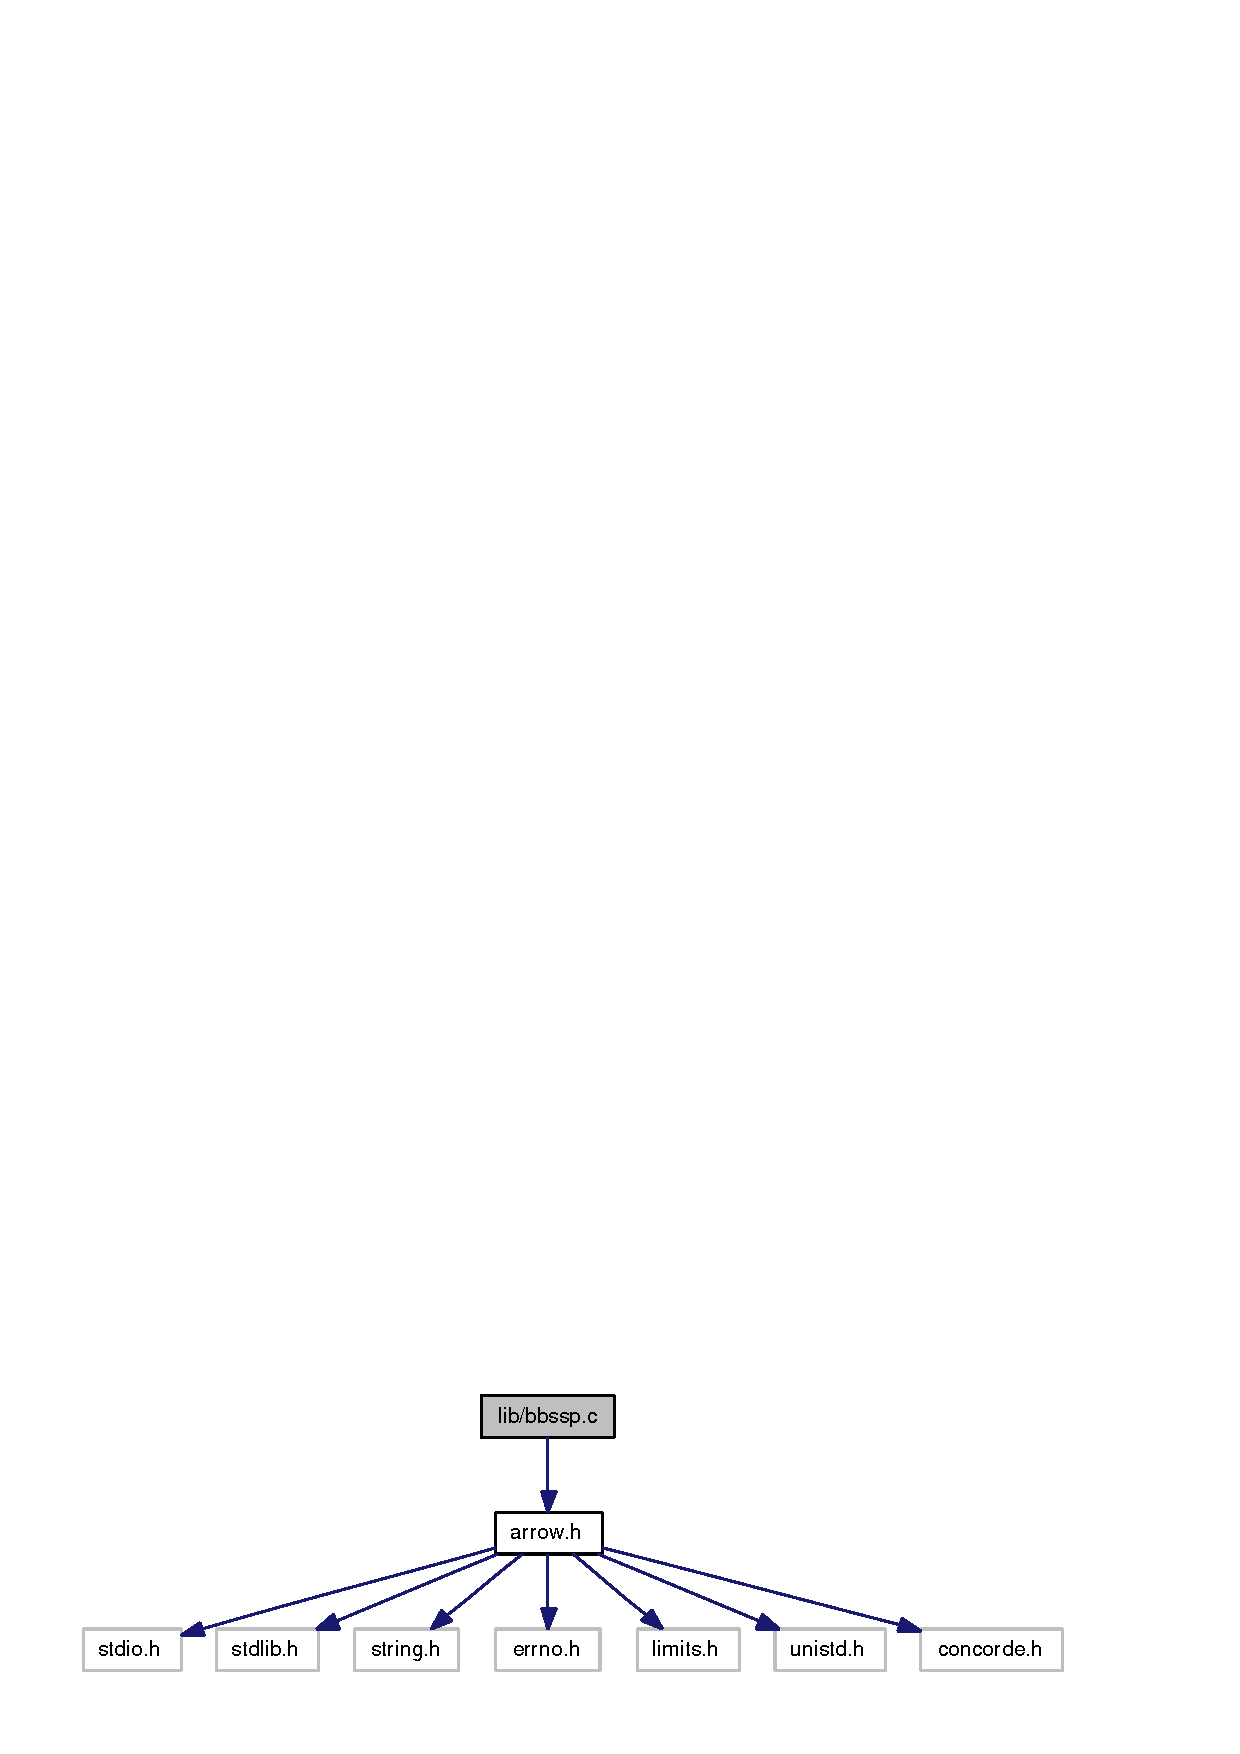
\includegraphics[width=257pt]{lib_2bbssp_8c__incl}
\end{center}
\end{figure}
\subsection*{Functions}
\begin{CompactItemize}
\item 
int \hyperlink{lib_2bbssp_8c_485f2a19b2a313bce3b255a845c8527d}{find\_\-art\_\-points} (\hyperlink{structarrow__problem}{arrow\_\-problem} $\ast$problem, int max\_\-cost, int node, int depth\_\-num, int root\_\-children, int $\ast$visited, int $\ast$depth, int $\ast$low, int $\ast$parent, int $\ast$art\_\-point)
\begin{CompactList}\small\item\em Recursively searches for articulation points in the graph using only costs less than or equal to 'max\_\-cost' out from the given node. \item\end{CompactList}\item 
int \hyperlink{lib_2bbssp_8c_d6098d008ef724a58c6960d8f28bf925}{arrow\_\-bbssp\_\-solve} (\hyperlink{structarrow__problem}{arrow\_\-problem} $\ast$problem, \hyperlink{structarrow__problem__info}{arrow\_\-problem\_\-info} $\ast$info, \hyperlink{structarrow__bbssp__result}{arrow\_\-bbssp\_\-result} $\ast$result)
\begin{CompactList}\small\item\em Solves the bottleneck biconnected spanning subgraph problem (BBSSP) on the given problem. \item\end{CompactList}\item 
int \hyperlink{lib_2bbssp_8c_727cb19dd9cfa6315e1155796daef833}{arrow\_\-bbssp\_\-biconnected} (\hyperlink{structarrow__problem}{arrow\_\-problem} $\ast$problem, int max\_\-cost, int $\ast$result)
\begin{CompactList}\small\item\em Determines if the graph is biconnected using only edges with costs less than or equal to the given value. \item\end{CompactList}\end{CompactItemize}


\subsection{Detailed Description}
Bottleneck biconnected spanning subgraph problem implemenation. 

Implemenation of the bottleneck biconnected spanning subgraph problem (BBSSP) that's used as a lower bound for the Bottleneck TSP objective value.

\begin{Desc}
\item[Author:]John LaRusic \end{Desc}


Definition in file \hyperlink{lib_2bbssp_8c-source}{bbssp.c}.

\subsection{Function Documentation}
\hypertarget{lib_2bbssp_8c_727cb19dd9cfa6315e1155796daef833}{
\index{lib/bbssp.c@{lib/bbssp.c}!arrow\_\-bbssp\_\-biconnected@{arrow\_\-bbssp\_\-biconnected}}
\index{arrow\_\-bbssp\_\-biconnected@{arrow\_\-bbssp\_\-biconnected}!lib/bbssp.c@{lib/bbssp.c}}
\subsubsection{\setlength{\rightskip}{0pt plus 5cm}int arrow\_\-bbssp\_\-biconnected ({\bf arrow\_\-problem} $\ast$ {\em problem}, \/  int {\em max\_\-cost}, \/  int $\ast$ {\em result})}}
\label{lib_2bbssp_8c_727cb19dd9cfa6315e1155796daef833}


Determines if the graph is biconnected using only edges with costs less than or equal to the given value. 

\begin{Desc}
\item[Parameters:]
\begin{description}
\item[{\em problem}]\mbox{[}in\mbox{]} problem data \item[{\em max\_\-cost}]\mbox{[}in\mbox{]} value to check biconnectivity question against \item[{\em result}]\mbox{[}out\mbox{]} ARROW\_\-TRUE if biconnected, ARROW\_\-FALSE otherwise. \end{description}
\end{Desc}


Definition at line 88 of file bbssp.c.

References ARROW\_\-ERROR\_\-FATAL, ARROW\_\-FALSE, ARROW\_\-TRUE, arrow\_\-util\_\-create\_\-int\_\-array(), find\_\-art\_\-points(), and arrow\_\-problem::size.

Referenced by arrow\_\-bbssp\_\-solve().\hypertarget{lib_2bbssp_8c_d6098d008ef724a58c6960d8f28bf925}{
\index{lib/bbssp.c@{lib/bbssp.c}!arrow\_\-bbssp\_\-solve@{arrow\_\-bbssp\_\-solve}}
\index{arrow\_\-bbssp\_\-solve@{arrow\_\-bbssp\_\-solve}!lib/bbssp.c@{lib/bbssp.c}}
\subsubsection{\setlength{\rightskip}{0pt plus 5cm}int arrow\_\-bbssp\_\-solve ({\bf arrow\_\-problem} $\ast$ {\em problem}, \/  {\bf arrow\_\-problem\_\-info} $\ast$ {\em info}, \/  {\bf arrow\_\-bbssp\_\-result} $\ast$ {\em result})}}
\label{lib_2bbssp_8c_d6098d008ef724a58c6960d8f28bf925}


Solves the bottleneck biconnected spanning subgraph problem (BBSSP) on the given problem. 

\begin{Desc}
\item[Parameters:]
\begin{description}
\item[{\em problem}]\mbox{[}in\mbox{]} problem data \item[{\em result}]\mbox{[}out\mbox{]} BBSSP solution \end{description}
\end{Desc}


Definition at line 44 of file bbssp.c.

References arrow\_\-bbssp\_\-biconnected(), ARROW\_\-ERROR\_\-FATAL, ARROW\_\-SUCCESS, ARROW\_\-TRUE, arrow\_\-util\_\-zeit(), arrow\_\-problem\_\-info::cost\_\-list, arrow\_\-problem\_\-info::cost\_\-list\_\-length, arrow\_\-bbssp\_\-result::obj\_\-value, and arrow\_\-bbssp\_\-result::total\_\-time.

Referenced by main().\hypertarget{lib_2bbssp_8c_485f2a19b2a313bce3b255a845c8527d}{
\index{lib/bbssp.c@{lib/bbssp.c}!find\_\-art\_\-points@{find\_\-art\_\-points}}
\index{find\_\-art\_\-points@{find\_\-art\_\-points}!lib/bbssp.c@{lib/bbssp.c}}
\subsubsection{\setlength{\rightskip}{0pt plus 5cm}int find\_\-art\_\-points ({\bf arrow\_\-problem} $\ast$ {\em problem}, \/  int {\em max\_\-cost}, \/  int {\em node}, \/  int {\em depth\_\-num}, \/  int {\em root\_\-children}, \/  int $\ast$ {\em visited}, \/  int $\ast$ {\em depth}, \/  int $\ast$ {\em low}, \/  int $\ast$ {\em parent}, \/  int $\ast$ {\em art\_\-point})}}
\label{lib_2bbssp_8c_485f2a19b2a313bce3b255a845c8527d}


Recursively searches for articulation points in the graph using only costs less than or equal to 'max\_\-cost' out from the given node. 

\begin{Desc}
\item[Parameters:]
\begin{description}
\item[{\em problem}]\mbox{[}in\mbox{]} problem data structure \item[{\em max\_\-cost}]\mbox{[}in\mbox{]} the largest cost to consider as being in the graph \item[{\em node}]\mbox{[}in\mbox{]} the node to search outward from \item[{\em depth\_\-num}]\mbox{[}in\mbox{]} level at which the given node was first discovered \item[{\em root\_\-children}]\mbox{[}in\mbox{]} count of the number of children of the root \item[{\em visited}]\mbox{[}out\mbox{]} indicates if a node has been visited or not \item[{\em depth}]\mbox{[}out\mbox{]} indicates the discovery depth of a node \item[{\em low}]\mbox{[}out\mbox{]} indicates a back edge for some descendent of a node (e.g. the discovery depth of the node closest to the root and reachable from the given node by following zero or more edges downward and then at most one back edge) \item[{\em parent}]\mbox{[}out\mbox{]} indicates the closest \char`\"{}parent\char`\"{} of a node \item[{\em art\_\-point}]\mbox{[}out\mbox{]} indicates if the node is an articulation point \end{description}
\end{Desc}


Definition at line 162 of file bbssp.c.

References ARROW\_\-SUCCESS, arrow\_\-problem::get\_\-cost, and arrow\_\-problem::size.

Referenced by arrow\_\-bbssp\_\-biconnected().